\documentclass[fleqn,12pt]{article}
\usepackage[top=2cm, left=2cm,right=3cm,bottom=2cm]{geometry}
%\usepackage[fleqn]{amsmath}
\usepackage{amsmath}
\usepackage{url,enumerate}
\usepackage{color,hyperref,enumerate,multicol}
\usepackage{ifthen}
\newboolean{answers}
%\setboolean{answers}{true}  % set to true to include TODO statements
\setboolean{answers}{false}  % set to false to use input statements
\usepackage{amssymb}
\usepackage{tikz}
\newcommand{\<}{\ensuremath{\langle}}
\renewcommand{\>}{\ensuremath{\rangle}}
\newcommand{\Z}{\ensuremath{\mathbb{Z}}}
\newcommand{\N}{\ensuremath{\mathbb{N}}}
\newcommand{\ur}{\ensuremath{\underline{\mathrm{r}}}}
\newcommand{\uT}{\ensuremath{\underline{\mathrm{T}}}}
\newcommand{\uF}{\ensuremath{\underline{\mathrm{F}}}}
\newcommand{\uN}{\ensuremath{\underline{\mathrm{N}}}}
\newcommand{\ui}{\ensuremath{\underline{\mathrm{i}}}}
\newcommand{\uj}{\ensuremath{\underline{\mathrm{j}}}}
\newcommand{\ua}{\ensuremath{\underline{\mathrm{a}}}}
\newcommand{\ub}{\ensuremath{\underline{\mathrm{b}}}}
\newcommand{\un}{\ensuremath{\underline{\mathrm{n}}}}
\newcommand{\uv}{\ensuremath{\underline{\mathrm{v}}}}
\newcommand{\ba}{\ensuremath{\mathbf{a}}}
\newcommand{\bv}{\ensuremath{\mathbf{v}}}
\newcommand{\bb}{\ensuremath{\mathbf{b}}}
\newcommand{\bc}{\ensuremath{\mathbf{c}}}
\newcommand{\bi}{\ensuremath{\mathbf{i}}}
\newcommand{\bj}{\ensuremath{\mathbf{j}}}
\newcommand{\dotsize}{1pt}
\begin{document}
%\thispagestyle{empty}
\pagestyle{empty}
%\fontsize{11.5}{13.8}
% \fontsize{14}{17}
% \selectfont
\noindent {\bf MATH 301 - Section B}
\hfill {\bf Fall 2014}
\begin{center}
{\bf Midterm Exam}
\thispagestyle{empty}
%% covers sections 5.1--5.5 and 7.1--7.4
\end{center}
\vskip1cm
\noindent {\bf RULES}
\begin{enumerate}
\item All phones and other electronic devices must be silenced for the duration
  of the exam.
\item No books, notes, or calculators allowed.
\item Out of consideration for your classmates, do not make
disturbing noises during the exam. If you need a tissue, please ask for one.
\item Are you still reading the rules?  Did you read rule number 1?  If you
  haven't yet taken out your phone to turn it off, read rule
  number 1 a few more times.
\end{enumerate}
\vskip1cm
{\it Cheating will not be tolerated.}  If there are any indications that a
  student may have given or received unauthorized aid on this exam, the case 
  will be brought to the ISU Office of Academic Integrity.% \\
\\[4pt]
After finishing the exam, please sign the following statement
acknowledging that you understand and accept this policy:\\
\\
``On my honor as a student I,
\underline{\phantom{XXXXXXXXXXXXXXXX}}, have neither
given nor received unauthorized aid on this exam.''
\hbox{} \hskip .75cm {\small (print name clearly)}\\
\\
\begin{flushright} Signature: \underline{\phantom{XXXXXXXXXXXXXXXXXXXXXXXX}}
  Date: \underline{\phantom{XXXXXXXXXX}}
\end{flushright}

\begin{center}
  
{\bf Do not sign the pledge until after you have finished the exam.}
\end{center}

\newpage

\begin{enumerate}[{\bf 1.}]
\item Give precise definitions of the following:

  \begin{enumerate}
  %% \item {\bf algebra}

  %%   \vskip4cm

  \item {\bf semigroup}

    \vskip4cm

  \item {\bf monoid}

    \vskip4cm

  \item {\bf group}

    \vskip4.5cm

  \item {\bf abelian group}

    \vskip3.5cm

  \item {\bf cyclic group}
    
  \end{enumerate}

\newpage

\item Let $G$ denote the symmeteries of an equilateral triangle.

\begin{center}
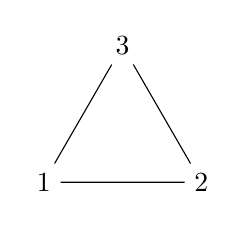
\begin{tikzpicture}[scale=0.5]
  \node (1) at (-2,0) {1};
  \node (2) at (2,0) {2};
  \node (3) at (0,3.4641) {3};
  \draw (1) to (2) to (3) to (1);
\end{tikzpicture}
\end{center}


  \begin{enumerate}
\item List the elements of this group using cycle notation.
\vskip7cm

\item What is the order of this group?
\vskip3cm
%%   %% \item What is the \emph{universe} of the group $G$?
%%   %% \item What is the set $X$ upon which the elements of $G$ act?
%%   \item Write down the Cayley table for this groupff. (This will be easier if you give
%%     short names to each of the group elements in part (a).)

%% \vskip5mm
%%     \begin{tabular}{c|c}
%% &\\
%% \phantom{XX}      & \phantom{XXXXXXXXXXXXXXXXXXXXXXXX}\\
%% \hline
%% &\\
%% &\\
%% &\\
%% &\\
%% &\\
%% &\\
%% &\\
%% &\\
%% &\\
%% &\\
%% &
%%     \end{tabular}
%% \vskip1cm 
\item Is this group cyclic? Is it abelian?\\
  (Give a brief justification for your answers. You may cite 4(b).)

  \end{enumerate}
\newpage

\item Suppose $H$ and $K$ are subgroups of a group $G$. Prove or disprove the following:
  \begin{enumerate}
  \item $H\cap K$ is a subgroup of $G$.
\vskip11cm
  \item $H\cup K$ is a subgroup of $G$.
  \end{enumerate}
\newpage

\item %Let $\mathbf{G} = \<G, \cdot, ^{-1}, e\>$ 
  Let $G$ be a group.  Prove the following:
  \begin{enumerate}
  \item $G$ is abelian if and only if $(gh)^2 = g^2h^2$ holds for all $g, h \in G$. \\
    {\it Proof:}
    \vskip7cm
  \item If $G$ is cyclic, then $G$ is abelian.\\
    {\it Proof:}
    \vskip6cm
  \item Give a specific example of a group $G$ and elements $g, h \in G$ for which $(gh)^2 \neq g^2h^2$. \\
    (Justify your answer.)
    \vskip4cm
  \item Give a specific example of a group that is abelian but not cyclic.\\
    (No justification necessary.)
  \end{enumerate}

\newpage
\item This problem has several parts.
First, state the following (without proof):
  \begin{enumerate}
  \item \emph{The Well Ordering Principle.} (about subsets of natural numbers)
    \vskip3cm

  \item \emph{The Division Algorithm.} (about integers $a$ and $b$ where $b>0$)
  \end{enumerate}
  \vskip3cm

Prove that every subgroup of a cyclic group is cyclic by following the
steps below.
First, let $G = \<a\>$ be a cyclic group and fix an arbitrary subgroup $H\leq G$.
  \begin{enumerate}
  \item Suppose $H$ contains only the identity, $e$. Say why $H$
    must be cyclic in this case. (one line/sentence)
    \vskip3cm
  \item Suppose instead that $H$ contains more than just the identity element. 
    Let $m$ be the smallest positive integer such that $a^m\in H$.  
    Why does such a number $m$ exists? (Hint: consider the set 
    $\{m \in \N: a^m \in H\}$; cite a well known principle; say
    why it applies here.)
    \vskip5cm
  \item Finally, prove the {\bf Claim} stated on the {\bf next page}. $\rightarrow$ \\
    (which says that $a^m$ generates $H$, where $m$ is the number from part (b)).
    %% ; that is, prove that if $x$ is an arbitrary element of $H$, then
    %%     $x$ is a power of $a^m$.
  \end{enumerate}

\newpage
{\bf Claim:} If $H\leq G = \<a\>$ and $m$ is the smallest positive integer such
that $a^m \in H$, then $H = \<a^m\>$.

\medskip

\noindent {\it Proof:}

\hfill

%% \newpage

%% \item
%%   Prove {\bf one} of the statements below. Only one answer will be graded.  (If
%%   you give more than one proof, then clearly label the one you want graded.)

%%   \begin{enumerate}
%% \item The order of an element of a cyclic group divides the order of the group.\\
%% (Do not simply cite Lagrange's Theorem.)

%% \item 
%% If $G = \<a\>$ is a cyclic group, then 
%% the subgroup $\<a^j, a^k\>$ generated by $a^j$ and $a^k$ is equal to
%% $\<a^d\>$, where $d = \gcd(j,k)$.
%% (Hint: Recall that there exist integers $r$ and $s$ such that $d = rm + sk$; you
%% may use this fact without proving it.)

%% \end{enumerate}
\newpage
\item
  Answer either (a) or (b). Only one answer will be graded.  (If
  you answer both, then clearly mark which should be graded.)
  \begin{enumerate}
\item 
Show that, for any cyclic group $G = \<a\>$, 
the subgroup $\<a^j, a^k\>$ generated by $a^j$ and $a^k$ is equal to
$\<a^d\>$, where $d = \gcd(j,k)$.
(Hint: Recall that there exist integers $r$ and $s$ such that $d = rm + sk$; you
may use this fact without proving it.)
\item
Show that for any group $G$, and any fixed element $g \in G$,
the map $\lambda_g : G \rightarrow G$ defined by
$\lambda_g(a) = g a$ is a permutation of $G$.
Then show that the order of the alternating group on $n$ letters is $|A_n| = n!/2$.
%% (Hint: first explain why the order of $S_n$ is $n!$, then prove that exactly half
%% of the elements of $S_n$ must be in $A_n$.)
\end{enumerate}

\newpage
\item
  \begin{enumerate}[(a)]
  \item Give a precise definition of \emph{equivalence relation}, then give an example.
    \vskip5cm
  \item Give a precise definition of \emph{partial order relation}, then give an example.
    \vskip5cm
    \item Let $f:X \rightarrow Y$ be a function and define the relation $\sim$
      on the set $X$ as follows:
    \[
    m \sim n \quad \text{ if and only if } \quad f(m) = f(n)
    \]
    What kind of relation is $\sim$?  (Justify your answer by checking the properties.)
  %% \item Give a precise definition of \emph{total order relation}, then give an example.
  %%   \vskip4cm
  %%   \item Of the three types of relations mentioned above, which of these is
  %%     typically associated with a partition of a set into disjoint subsets?
  %%   \vskip4cm
  \end{enumerate}

\newpage
\end{enumerate}
\begin{center}
  Extra Credit
\end{center}
\begin{enumerate}
\item[EC 1.] ($6$ points)
Below I have drawn the subgroup lattice diagrams for the groups $\Z_2$, $\Z_2 \times \Z_2$,
$\Z_7$, $\Z_{12}$, $\Z_{16}$, $\Z_{30}$, and $S_3$, but I've forgotten which diagram
go with which group.  I was able to label the first diagram
correctly.  If you think you can help me label the others, go for it. But
don't guess! 

\medskip

{\it $+1$ point for each correct answer, $-1/2$ point for each incorrect answer.} 
%\begin{multicols}{2}

\bigskip

\begin{center}
% Z_2
\begin{tikzpicture}[scale=1.25]
  \node (bot) at (0,0) [draw,circle,inner sep=1pt] {};
  \node (top) at (0,2) [draw,circle,inner sep=1pt] {};
  \draw (bot) to (top);
  \node (G) at (0,-1) {$G = \Z_2$};
  \node (line) at (.1,-1.2) {\underline{\phantom{XXXXXXX}}};
\end{tikzpicture}
\hskip3cm
% Z_7
\begin{tikzpicture}[scale=1.25]
  \node (bot) at (0,0) [draw,circle,inner sep=1pt] {};
  \node (top) at (0,2) [draw,circle,inner sep=1pt] {};
  \draw (bot) to (top);
  \node (line) at (0,-1.2) {\underline{\phantom{XXXXXXX}}};
\end{tikzpicture}
% Z_16
\hskip3cm
\begin{tikzpicture}[scale=1.25]
  \node (bot) at (0,0) [draw,circle,inner sep=1pt] {};
  \node (1) at (0,1) [draw,circle,inner sep=1pt] {};
  \node (top) at (0,2) [draw,circle,inner sep=1pt] {};
  \draw (bot) to (1) to (top);
  \node (line) at (0,-1.2) {\underline{\phantom{XXXXXXX}}};
\end{tikzpicture}
\end{center}
\vskip1cm
\begin{center}
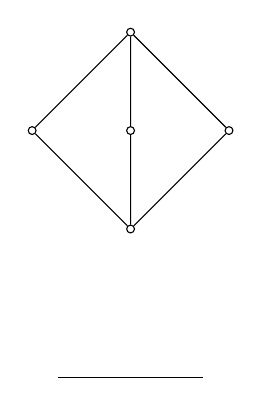
\begin{tikzpicture}[scale=1.25]
  \node (bot) at (0,0) [draw,circle,inner sep=1pt] {};
  \node (1) at (1,1) [draw,circle,inner sep=1pt] {};
  \node (2) at (-1,1) [draw,circle,inner sep=1pt] {};
  \node (3) at (0,1) [draw,circle,inner sep=1pt] {};
  \node (top) at (0,2) [draw,circle,inner sep=1pt] {};
  \draw (bot) to (1) to (top) to (2) to (bot) to (3) to (top);
  \node (line) at (0,-1.4) {\underline{\phantom{XXXXXXX}}};
\end{tikzpicture}
\hskip3cm
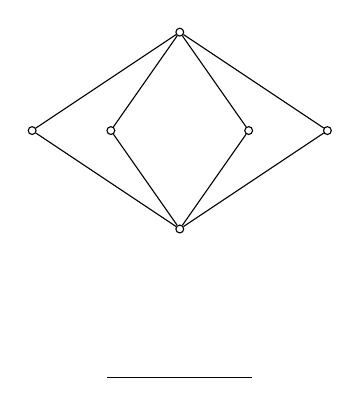
\begin{tikzpicture}[scale=1.25]
  \node (bot) at (0,0) [draw,circle,inner sep=1pt] {};
  \node (1) at (1.5,1) [draw,circle,inner sep=1pt] {};
  \node (2) at (-1.5,1) [draw,circle,inner sep=1pt] {};
  \node (3) at (.7,1) [draw,circle,inner sep=1pt] {};
  \node (4) at (-.7,1) [draw,circle,inner sep=1pt] {};
  \node (top) at (0,2) [draw,circle,inner sep=1pt] {};
  \draw (bot) to (1) to (top) to (2) to (bot) to (3) to (top) to (4) to (bot);
  \node (line) at (0,-1.4) {\underline{\phantom{XXXXXXX}}};
%  \node (G) at (0,-1.5) {$G =$};
\end{tikzpicture}
\end{center}
\vskip1cm
\begin{center}
\begin{tikzpicture}[scale=0.7]
  \node (1) at (0,0) [draw,circle,inner sep=1pt] {};
  \node (6) at (2,2)[draw,circle,inner sep=1pt] {}; 
  \node (4) at (-2,2) [draw,circle,inner sep=1pt] {};
  \node (2) at (0,4) [draw,circle,inner sep=1pt] {};
  \node (3) at (4,4) [draw,circle,inner sep=1pt] {};
  \node (G) at (2,6) [draw,circle,inner sep=1pt] {};
  \draw (1) to (6) to (2) to (4) to (1);
  \draw (6) to (3) to (G) to (2) to (4);
  \node (line) at (1,-1.4) {\underline{\phantom{XXXXXXX}}};
%  \node (G) at (0,-1.5) {$G =$};
\end{tikzpicture}
\hskip3cm
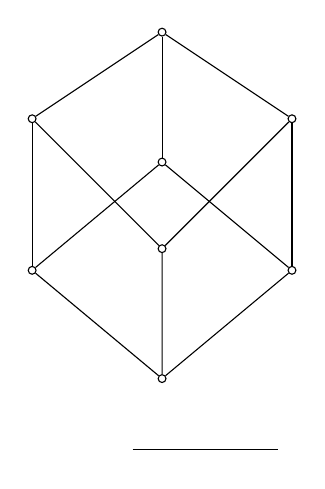
\begin{tikzpicture}[scale=0.55]
  \node (e) at (0,0)  [draw,circle,inner sep=1pt] {};
  \node (G) at (0,8) [draw,circle,inner sep=1pt] {};
  \node (2) at (-3,6) [draw,circle,inner sep=1pt] {};
  \node (3) at (0,5)  [draw,circle,inner sep=1pt] {};
  \node (5) at (3,6) [draw,circle,inner sep=1pt] {}; 
  \node (6) at (-3,2.5) [draw,circle,inner sep=1pt] {};
  \node (10) at (0,3)  [draw,circle,inner sep=1pt] {};
  \node (15) at (3,2.5)  [draw,circle,inner sep=1pt] {};
  \node (line) at (1,-1.4) {\underline{\phantom{XXXXXXX}}};
  \draw (e) to (15) to (3) to (6) to (e);
  \draw (e) to (10) to (5) to (G) to (2) to (10);
  \draw (6) to (2) (3) to (G) (15) to (5);
\end{tikzpicture}
\end{center}

\item[EC 2.] (1/2 point) Which group appears in William DeMeo's GitHub gravatar?\\
{\small (William DeMeo the mathematician, not the actor.)}
\end{enumerate}

\end{document}


\begin{tikzpicture}[scale=0.75]
  \node (1) at (0,0) {$\langle e \rangle$}; 
  \node (6) at (2,2) {$\langle g^6 \rangle$}; 
  \node (4) at (-2,2) {$\langle g^4 \rangle$}; 
  \node (2) at (0,4) {$\langle g^2 \rangle$}; 
  \node (3) at (4,4) {$\langle g^3 \rangle$}; 
  \node (G) at (2,6) {$\langle g \rangle$}; 
  \draw (1) to (6) to (2) to (4) to (1);
  \draw (6) to (3) to (G) to (2) to (4);
  \node (line) at (1,-1.4) {\underline{\phantom{XXXXXXX}}};
%  \node (G) at (0,-1.5) {$G =$};
\end{tikzpicture}

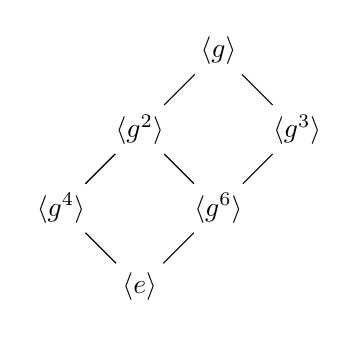
\begin{tikzpicture}[scale=0.5]
  \node (1) at (0,0) {$\langle e \rangle$}; 
  \node (6) at (2,2) {$\langle g^6 \rangle$}; 
  \node (4) at (-2,2) {$\langle g^4 \rangle$}; 
  \node (2) at (0,4) {$\langle g^2 \rangle$}; 
  \node (3) at (4,4) {$\langle g^3 \rangle$}; 
  \node (G) at (2,6) {$\langle g \rangle$}; 
  \draw (1) to (6) to (2) to (4) to (1);
  \draw (6) to (3) to (G) to (2) to (4);
\end{tikzpicture}

\begin{center}
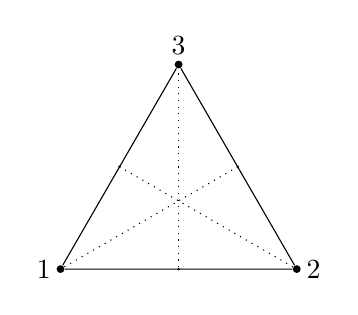
\begin{tikzpicture}[scale=0.75]
  \node (0) at (0,0) [fill,circle,inner sep=.2pt] {};
  \node (1) at (-2,0) [fill,circle,inner sep=1pt] {};
  \node (2) at (2,0) [fill,circle,inner sep=1pt] {};
  \node (3) at (0,3.4641) [fill,circle,inner sep=1pt] {};
  \node (4) at (1, 1.732) [fill,circle,inner sep=.2pt] {};
  \node (5) at (-1, 1.732) [fill,circle,inner sep=.2pt] {};
  \draw (1) node [left] {$1$};
  \draw (2) node [right] {$2$};
  \draw (3) node [above] {$3$};
  \draw (1) to (2) to (3) to (1);
  \draw[dotted] (0) to (3);
  \draw[dotted] (1) to (4);
  \draw[dotted] (2) to (5);
\end{tikzpicture}
\end{center}


\item
  \begin{enumerate}[(a)]
    \item Let $f:X \rightarrow Y$ be a function and define the relation $\sim$
      on the set $X$ as follows:
    \[
    m \sim n \quad \text{ if and only if } \quad f(m) = f(n)
    \]
    What kind of relation is $\sim$?  (Justify your answer by checking the properties.)
    \vskip10cm
  \item Does $\sim$ induce a partition of $X$ into disjoint sets?  If so,
    describe the sets in the partition.  If not, say why not.
  \end{enumerate}

\newpage


